\chapter{Industrial ODS Concept\label{cha:chapter3}}

In this concept the ODS is a recipe for an OPC Vision server. See fig. \ref{fig:concept} for an overview. 
\begin{figure}
    \centering
    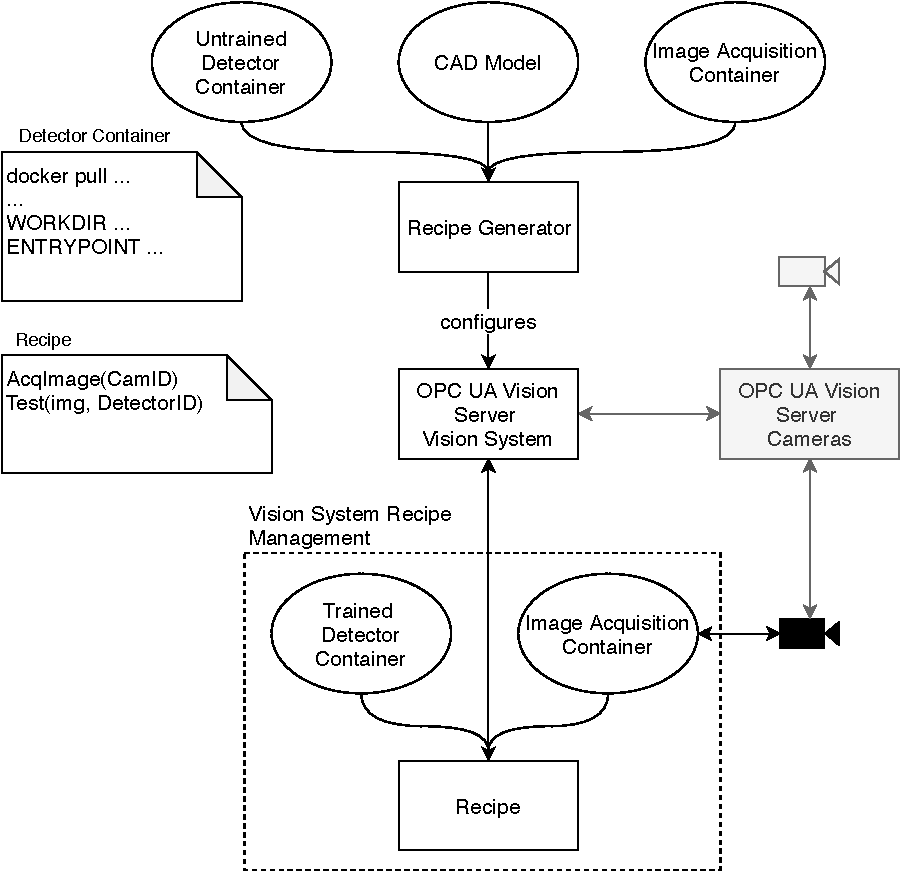
\includegraphics[width=\textwidth]{img/Concept.pdf}
    \caption[Concept]{Illustration of the industrial ODS concept. Ellipses denote inputs, solid rectangles systems, dotted rectangles scopes of systems and notes the content of a file. The OPC UA Vision server for cameras is not yet released by the OPC foundation, hence marked grey.}
    \label{fig:concept}
\end{figure}

The ODS is a trained detector container which is generated with a CAD model and an untrained detector as input. The detector must provide two methods:
\begin{tabbing}
\label{detectormethods}
    space \= space \= spacespacespace \= spacespacespacespace \= spacespacespace \kill
    \>  Train(\\
    \>  \>  (in)	 \> 	CADType          \> CADModel); \\
    \>  Test(\\
    \>  \>  (in)	 \> 	ImageType     \> Image\\
    \>  \>  (out)	 \> 	PoseType           \> Pose); 
\end{tabbing}

Train is a training routine which generates several views or templates from a CAD model. It must be preconfigured by the detector provider e.g. learning rates of neural networks have to be preset. After training the detector container includes generated templates or views and is callable with the Test method.  Test requires an image for processing the pose of an object aided by the generated templates.  Input and output types are not specified in this thesis. The container is illustrated as a Docker image, this is not mandatory however.

The detector container is added to recipe management of the VS via OPC UA Vision server. Recipes are scripts which handle image acquisition- and detection container calling and OPC UA Vision server interaction. Scripts can be added by the recipe generator or another entity. Image acquisition is currently set to be handled between image acquisition containers and cameras directly. This might change in the near future. During a phone interview conducted on 30th of April 2019, VDMA member Dr. Reinhard Heister stated that part 2 of the OPC Vision specification will direct the component layer. A component can be a camera that offers an OPC Vision server itself. For this task, OPC foundation and EMVA, supervisor of the GenICam interface \cite{LastvisitedMay4th20192019GenICamStandard} for cameras, will join forces. Hence in a few years time it will be possible to have the VS to be interoperable with any camera supporting OPC Vision and the images can be acquired via the OPC servers.


\section{Sequence Diagram}
Figs. \ref{fig:runtimeviewgen} and \ref{fig:runtimeviewexec} show an example sequence diagram of the service generation, transfer and execution. The approach is as follows:
\begin{figure}
    \centering
    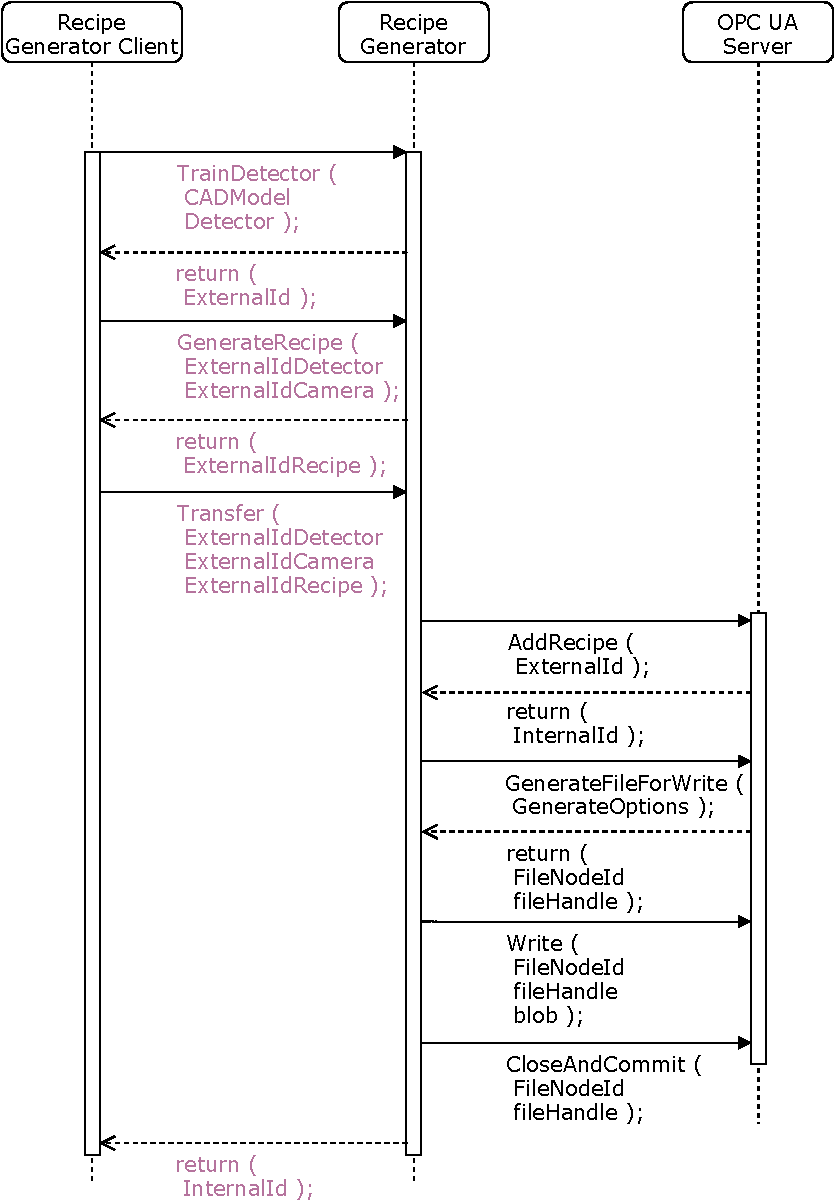
\includegraphics[height=0.9\textheight]{img/ConceptRuntimeView-RecipeGenerationAndTransfer.pdf}
    \caption[Sequence diagram recipe generation and method based transfer]{Sequence diagram of recipe generation and method based transfer to OPC UA Vision server. Pink arrows denote methods which are not covered by OPC Vision specification. Not all parameters of method signatures are shown.}
    \label{fig:runtimeviewgen}
\end{figure}

\begin{figure}
    \centering
    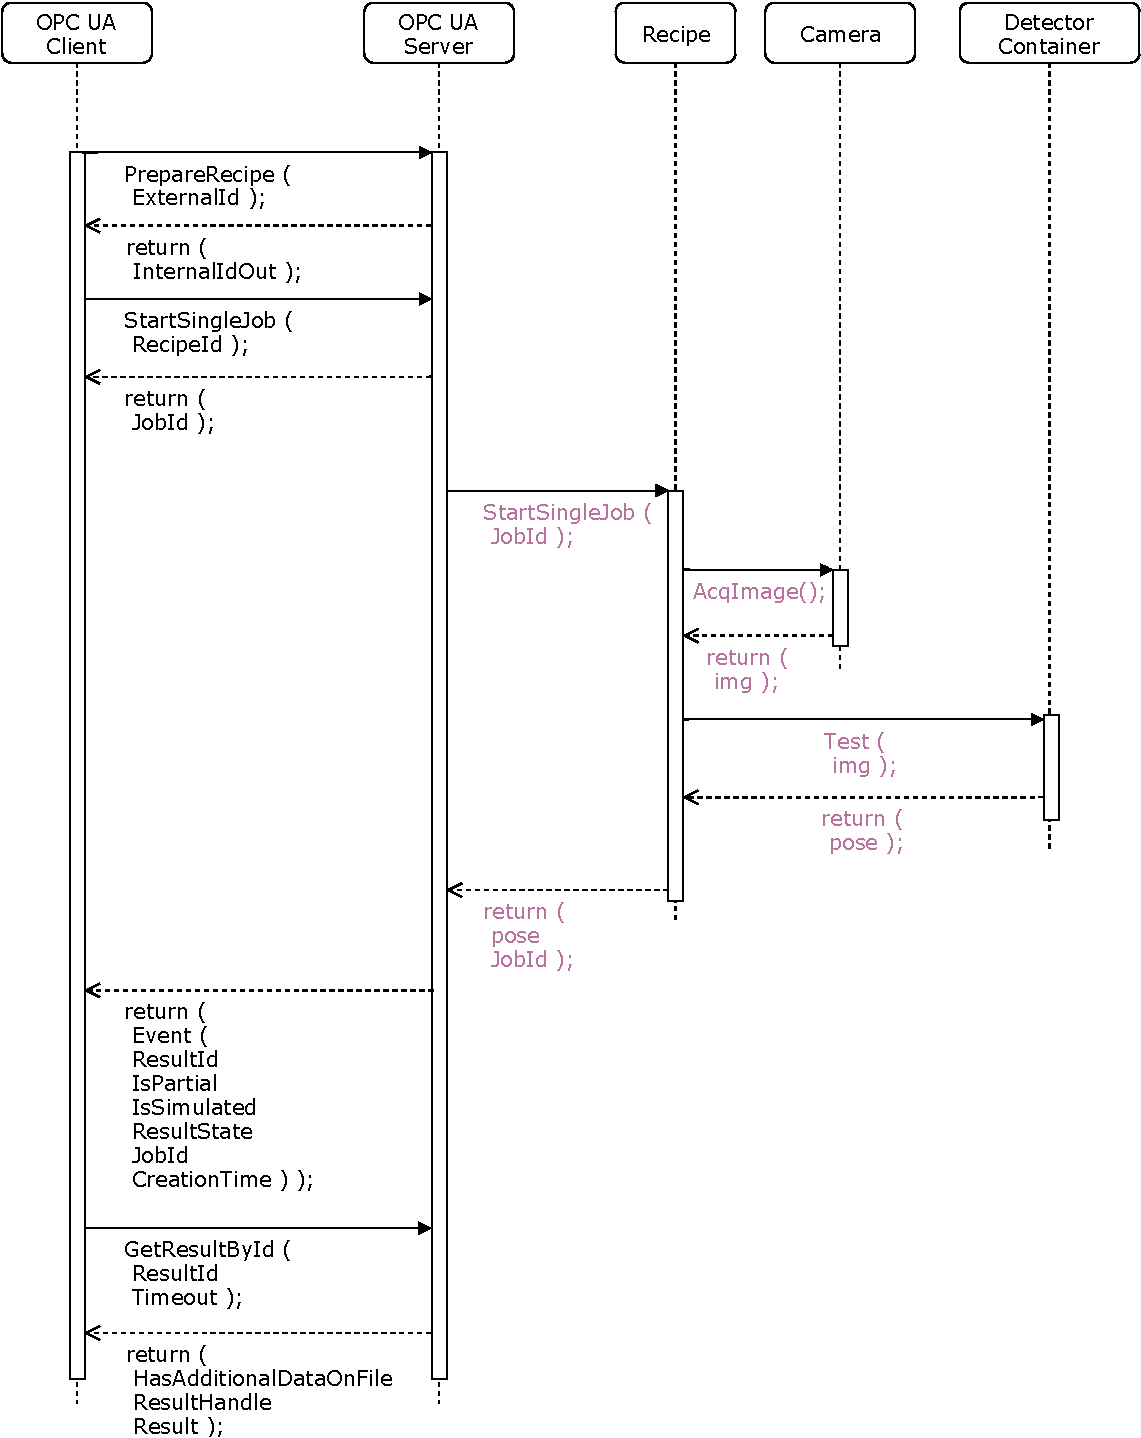
\includegraphics[height=0.9\textheight]{img/ConceptRuntimeView-RecipeExecution.pdf}
    \caption[Sequence diagram of recipe execution]{Sequence diagram of recipe execution of method based OPC UA Vision server. Pink arrows denote the recipe which is not covered by OPC Vision specification. Not all parameters of method signatures are shown.}
    \label{fig:runtimeviewexec}
\end{figure}

\begin{itemize}
    \item Generation and Transfer
    \begin{itemize}
        \item TrainDetector trains the detector with the Train method using a CAD model as input. The detector service changes state from untrained to trained and can be called via Test method.
        \item GenerateRecipe puts image acquisition and detector into sequence. Hence, when triggered an image is grabbed, passed to the Test method of the detector, which output the pose of the object in the image.
        \item Transfer initiates detector, image acquisition or recipe transfer. The object to be transferred is identified with the ExternalId.
        \item AddRecipe creates a new recipe opject and maps an InternalId to the ExternalId. ExternalId is an OPC UA datatype identifying a recipe in the view of the environment, InternalId is an OPC UA data type identifying an instance of the recipe on the VS.  InternalId is necessary because recipes can not only be handled via the server but also locally on the VS. For the OPC UA client, only the ExternalId should be callable and internal ambiguities must be handled by the VS. The created recipe object can contain meta data of the recipe and a reference to the recipe itself. As of now, it contains no data.
    	\item GenerateFileForWrite creates a new temporary file object. The GenerateOptions parameter contains the ExternalId of the process. The method returns a FileNodeId and a FileHandle. The temporary file object offers Write and CloseAndCommit methods to transfer binary recipe data. The recipe itself is treated as a file and is referenced in the recipe object.
    \end{itemize}
    \item Execution
    \begin{itemize}
    	\item PrepareRecipe is used to prepare a recipe so that it can be used for starting a job on the vision system. There are several ways the vision system can cope with recipes and their preparation. For example, the vision system can have several recipes prepared for immediate execution or just a single one. PrepareRecipe triggers transition from state Initialized to state Ready of the VS state machine. If the client tries to prepare a detector oder image acquisition container it should return an error.
    	\item StartSingleJob method triggers transition from state Ready to state SingleExecution. Parameter RecipeId is the ExternalId of the recipe script. The method returns a JobId which has to be used to query any information about the Job later.
    	\item AcqImage triggers a camera to acquire an image. In case several cameras are addressable, the method can be overloaded with a CameraId.
    	\item Test calls the detection routine of the detector service and returns the pose an object.
    	\item Once the Train method is complete the OPC server triggers an event to the OPC client containing the JobId and ResultId. It also provides information on whether the result is partial, the job is done and when the result was created.
    	\item GetResultById is used by the client to query the template matching result via RecipeId and a timeout which aborts the transfer after a given time. It returns meta data about the result and the possible reference to result data containing e.g. the base image. In this case, the detected point can be stored in the result object itself.
    \end{itemize}
\end{itemize}

\section{Deployment}
\subsection{Vision System}
In a typical industrial environment, the VS is a production line or a single machine. According to the OPC Vision specification the application can range from simple light barriers to complex pose detection. The recipes presented here are rather designed for the latter purpose, however can be used for the former, too. On the software side, the VS has to cover recipe, configuration and result management. Depending on the size of the system (number of cameras, data storage, CPU cores...) it can be deployed on a single industrial PC or in a larger factory cloud. The detection and image acquisition services in this work are containerized microservices, so the underlying hardware must support the containerization engine. According to an interview with VDMA experts \cite{Lastvisited26-04-20192015OPCVision} more and more machine vision functionalities shall be transferred to PLCs. This might call for a different approach of deployment for the recipes in a later stage. The OPC client triggering the job / recipe execution is usually a PLC.

\subsection{Recipe Generator}
As for the recipe generator, there are more possibilities. Since detectors could be added by several vendors in a hub, it would make sense to make this available in a (virtual private) cloud. The recipe generation might also require excessive computing power, which can be provided by cloud platforms. Furthermore, mobile networks such as the 5G technology offer a bandwidth up to 10.000\,MBit/s and a latency under 1\,ms, so costs on the infrastructure side can be minimized. Possible drawback is the increased security need of data storage and transmission.

The generator might also be deployed as part of the vision system. The advantages of this concept are better data protection possibilities and lower latency. The drawback in this case is the lower computing power and tougher access for ODS vendors.

\section{Interfaces}
\subsection{Detector Containers}
The detector containers are called during the execution of a recipe. The services might also be called in sequence. For this communication a standardized interface is of great help. As for the semantic, the two methods Train and Test are defined. For data transport RPC is a good choice due to its high performing request calls. With the Train and Test methods defined, most of the application logic can reside inside the server (detector container), hence changes of ODM do not cause changes for the client (recipe). The connection between recipe, OPC UA Vision server and cameras is implementation specific.

\subsection{Recipe Generator}
The recipe generator needs an interface for the OPC UA Vision server on the one hand and on the other hand for the recipe generator client. In case the generator is deployed in an industrial environment it would be reasonable to configure not only the recipe transfer but also the recipe generation via OPC UA to maintain a great interoperability within the shopfloor. For instance, CAD models can be created by cameras and automatically sent to the recipe generator. In case it is deployed in a web environment, an interface rather developed for web technologies is advantageous. For instance RPC with a RESTful adapter could be used for that purpose.

\subsection{Image Acquisition}
As of now, the image acquisition containers do not have a standardized interface. This is due to the plans of the OPC foundation of fulfilling this task in the near future.

\section{Orchestration of Recipe Management}
The recipe, image acquisition- and  detector containers combine to recipe management of the OPC UA Vision server. As recipes handle image acquisition and detector container calling, one could say it serves as an orchestrator and is a single point of failure. A possible hazard would be applying too much application logic to the recipe, thus it should stay simple and only run necessary OD steps by calling the containers in sequence with a standardized interface. This maximizes cohesion of the components. In case putting several trained detector containers in sequence, the output of the Test method would have to be abstracted since the second and following containers would receive a pose of an object as input which is unlikely useful. Abstracting output types would again shift application logic to the recipe which should be minimized. Hence, sequencing OD containers should be scoped in a container which handles the sequencing internally and is externally callable via Train \& Test methods.